

\begin{tikzpicture}[scale=1,solid,black,
	declare function={
		c(\x)= 4;	
		vol(\x)= 0 + and(\x>1,\x <= 5)*(\x-1) + and(\x > 5, \x <= 6)*4 + and(\x > 6, \x <=10)*(4-(\x-6)) + and(\x > 3,\x<4)*(.5*(\x-3)) + and(\x >= 4, \x <= 7)*.5 + and(\x > 7, \x <8)*(.5-.5*(\x-7));		
	}]
	
	
	\begin{axis}[xmin=0,xmax=10,ymax=5.5, ymin=0, samples=500,width=10cm,height=5cm,
		axis x line*=bottom, axis y line*=left, axis lines=middle, xtick={1,2,3,4,5,6,7,8,9,10},ytick={1,2,3,4,4.5},yticklabels={$1$,$2$,$3$,$4$,$4+\tfrac{1}{\lambda}\quad$}]
		\addplot[thick,domain=0:11,dashed] {c(x)} node[below,pos=.3]{$c_{e}$};
		\addplot[ultra thick,domain=0:11,blue] {vol(x)} node[above,pos=.5]{$x_{e}(h_\lambda,\emptyarg)$};
	\end{axis}

\end{tikzpicture}